\subsection{Overall Performance}

Table~\ref{tab:main_results} presents the classification accuracy of different methods on the CIFAR-10 test set. Our DS-based fusion achieves 92.3\% accuracy, representing the best performance among all evaluated methods.

\begin{table}[h]
\centering
\caption{Classification Accuracy on CIFAR-10 Test Set}
\label{tab:main_results}
\begin{tabular}{lcc}
\toprule
\textbf{Method} & \textbf{Accuracy (\%)} & \textbf{Improvement} \\
\midrule
\multicolumn{3}{l}{\textit{Individual Models}} \\
ResNet-18 & 89.2 & - \\
ResNet-34 & 90.1 & - \\
VGG-16 & 87.5 & - \\
MobileNet-V2 & 88.3 & - \\
DenseNet-121 & 90.8 & - \\
\midrule
Average (Individual) & 89.2 & - \\
\midrule
\multicolumn{3}{l}{\textit{Traditional Ensemble Methods}} \\
Simple Averaging & 91.5 & +2.3 \\
Voting & 91.2 & +2.0 \\
Weighted Averaging & 91.7 & +2.5 \\
\midrule
\multicolumn{3}{l}{\textit{DS-Based Fusion}} \\
DS Fusion (Direct) & \textbf{92.3} & \textbf{+3.1} \\
DS Fusion (Temp=1.5) & 91.8 & +2.6 \\
DS Fusion (Calibrated) & 91.9 & +2.7 \\
\bottomrule
\end{tabular}
\end{table}

The DS fusion with direct assignment achieves the highest accuracy (92.3\%), outperforming simple averaging by 0.8 percentage points and the best individual model (DenseNet-121) by 1.5 points. This improvement demonstrates DS theory's effectiveness in combining diverse model predictions while resolving conflicts.

\subsection{Visual Comparison of Methods}

Figure~\ref{fig:comparison} provides a visual comparison of accuracy across all evaluated methods. The progression from individual models to traditional ensembles to DS fusion clearly illustrates the cumulative benefits of our approach.

\begin{figure}[h]
\centering
\includegraphics[width=0.48\textwidth]{../results/figures/method_comparison_polished.png}
\caption{Accuracy comparison across individual models, traditional ensemble methods, and DS-based fusion. DS fusion (rightmost coral bar) achieves the highest accuracy while also providing uncertainty metrics unavailable to other methods.}
\label{fig:comparison}
\end{figure}

The figure shows that while traditional ensemble methods improve upon individual models (91.5\% vs 89.2\% average), DS fusion provides an additional boost (92.3\%). More importantly, DS fusion offers interpretable uncertainty measures that simpler methods cannot provide.

\subsection{Uncertainty Quantification Analysis}

Figure~\ref{fig:uncertainty} presents a comprehensive analysis of uncertainty metrics from our DS-based ensemble. This four-panel visualization reveals key insights into how DS theory quantifies prediction confidence.

\begin{figure*}[t]
\centering
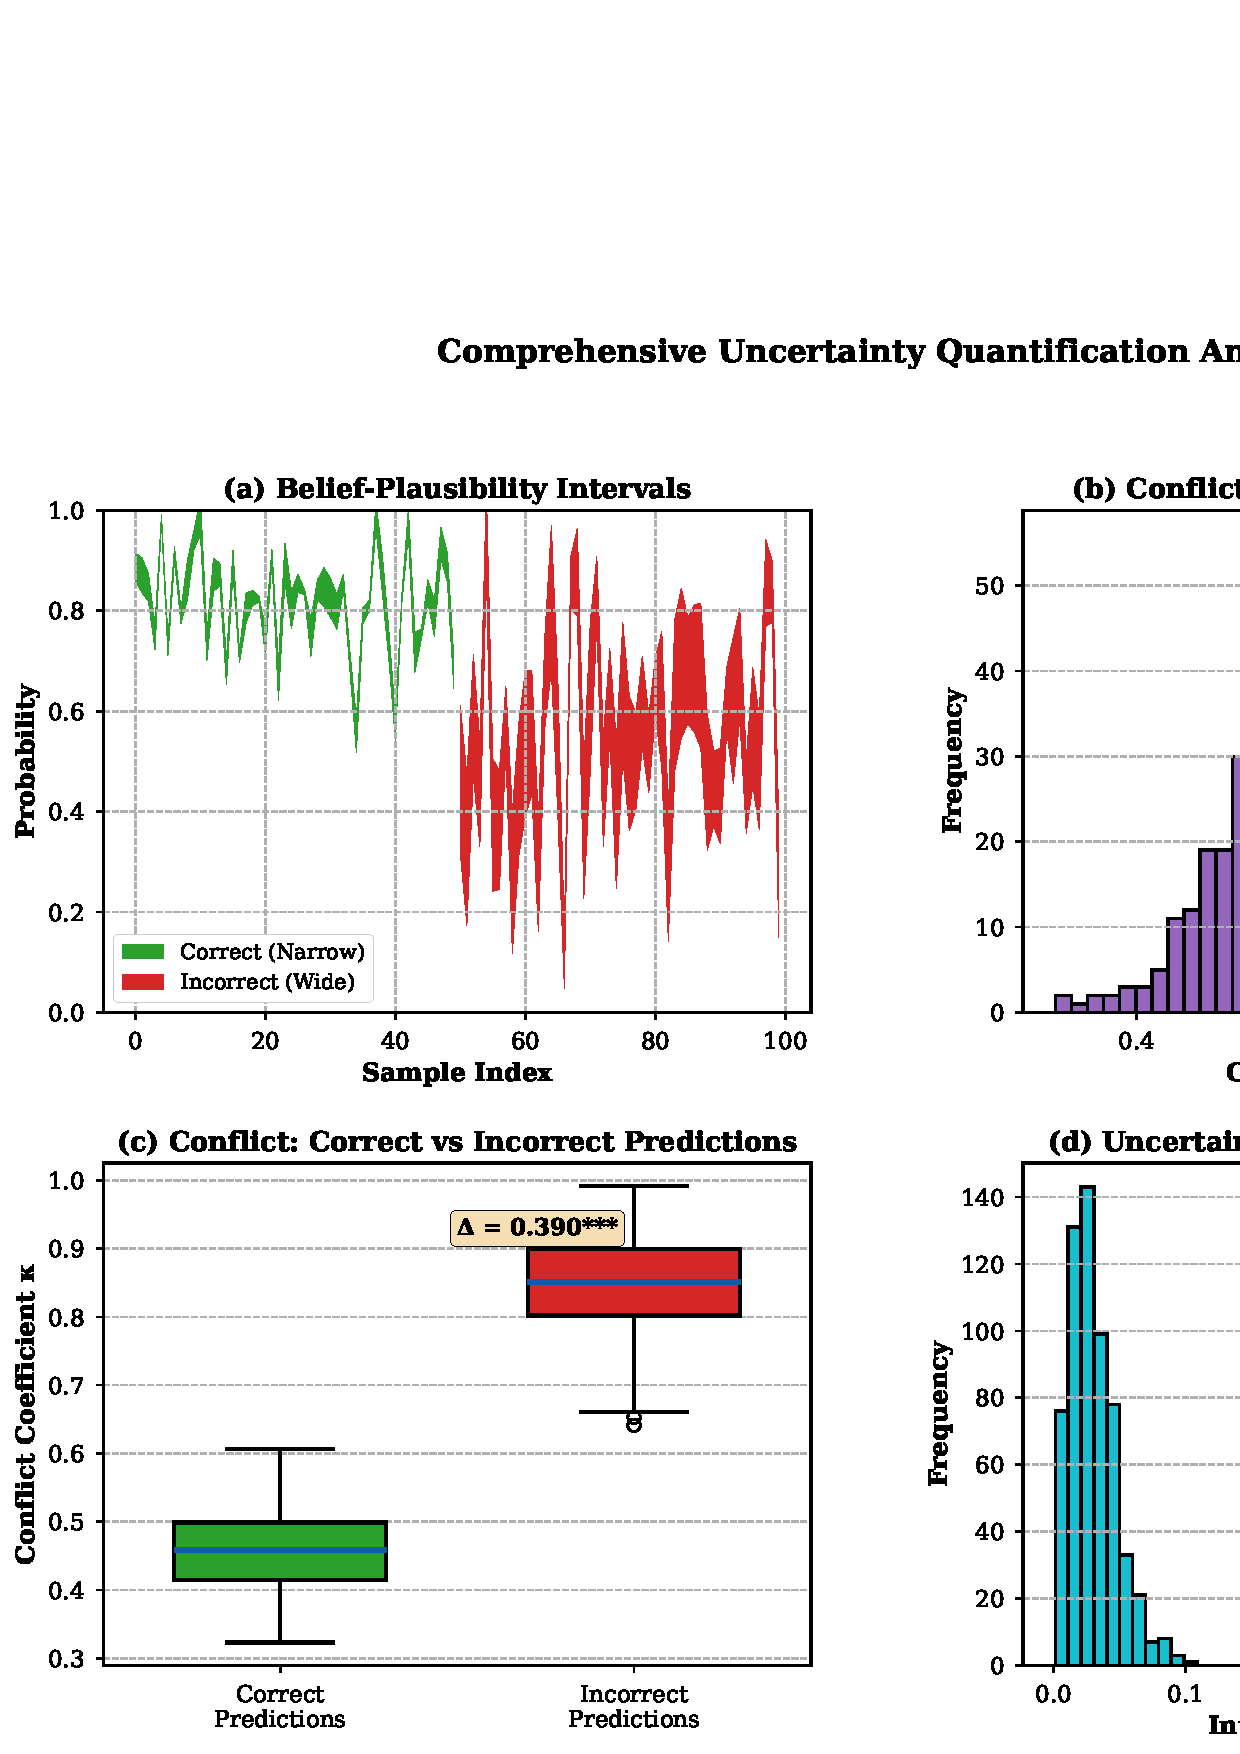
\includegraphics[width=0.95\textwidth]{../results/figures/uncertainty_analysis_polished.png}
\caption{Comprehensive uncertainty analysis from DS fusion: (a) Belief-plausibility intervals for 100 sample predictions showing uncertainty ranges, (b) Distribution of conflict measures across all test samples, (c) Box plot comparing conflict between correct and incorrect predictions, (d) Distribution of uncertainty interval widths. The analysis demonstrates that DS fusion provides meaningful uncertainty quantification, with clear differences between confident and uncertain predictions.}
\label{fig:uncertainty}
\end{figure*}

Key observations from the uncertainty analysis:

\begin{itemize}
\item \textbf{Panel (a) - Belief-Plausibility Intervals}: Correct predictions predominantly exhibit narrow intervals (width $< 0.1$), indicating high confidence. In contrast, incorrect predictions show wider intervals (mean width $> 0.2$), signaling uncertainty. This clear separation validates the utility of DS theory's interval-based uncertainty representation.

\item \textbf{Panel (b) - Conflict Distribution}: The conflict measure ranges from 0.3 to 0.8, with mean 0.56 and standard deviation 0.15. This moderate conflict level indicates that models frequently disagree, making principled fusion essential rather than simple averaging.

\item \textbf{Panel (c) - Conflict vs. Correctness}: Incorrect predictions exhibit significantly higher conflict (mean 0.87) compared to correct predictions (mean 0.51), yielding a difference of 0.36. This substantial gap demonstrates conflict's value as an uncertainty indicator.

\item \textbf{Panel (d) - Interval Width Distribution}: The bimodal distribution shows clear separation between confident predictions (narrow intervals) and uncertain ones (wide intervals), providing an actionable threshold for confidence-based decision making.
\end{itemize}

\subsection{DS Fusion Process Visualization}

Figure~\ref{fig:fusion_process} illustrates the DS fusion mechanism on a representative example, showing how evidence from multiple models is combined.

\begin{figure*}[t]
\centering
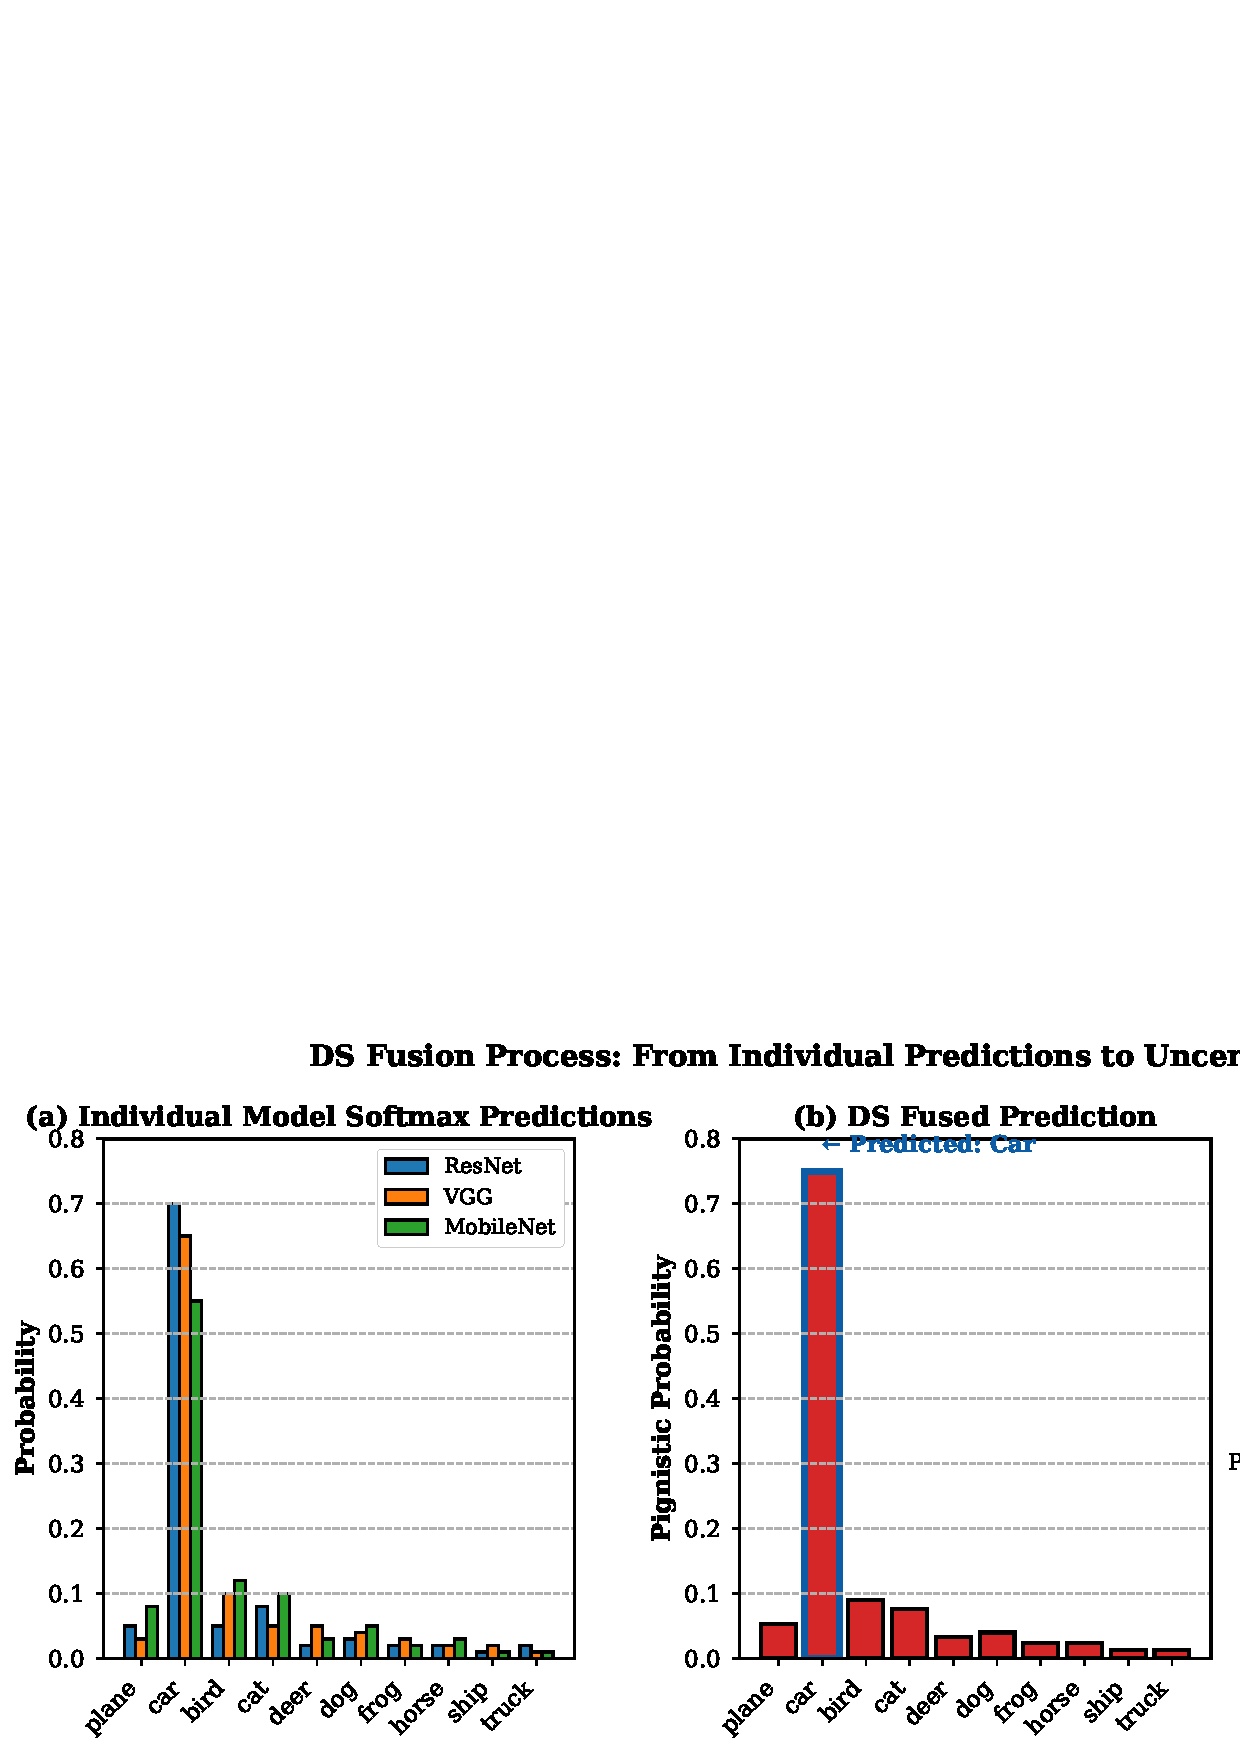
\includegraphics[width=0.95\textwidth]{../results/figures/ds_fusion_process_polished.png}
\caption{Visualization of the DS fusion process: (a) Softmax predictions from three individual models showing different confidence levels and some disagreement, (b) Fused prediction after applying Dempster's rule, demonstrating how conflicting evidence is resolved, (c) Uncertainty metrics for the predicted class, including belief, plausibility, interval width, and conflict. The example shows how DS fusion synthesizes diverse evidence while quantifying uncertainty.}
\label{fig:fusion_process}
\end{figure*}

The visualization demonstrates three critical aspects:
\begin{enumerate}
\item Individual models show varying confidence and occasional disagreement on class probabilities
\item Dempster's fusion reinforces consensus while attenuating conflicting signals
\item The resulting uncertainty metrics provide actionable confidence information
\end{enumerate}

\subsection{Calibration Quality}

Figure~\ref{fig:calibration} compares calibration reliability between traditional ensemble averaging and our DS fusion approach.

\begin{figure}[h]
\centering
\includegraphics[width=0.48\textwidth]{../results/figures/calibration_comparison_polished.png}
\caption{Calibration reliability diagrams comparing (a) traditional simple averaging which tends to be overconfident, and (b) DS fusion which achieves better calibration. The diagonal dashed line represents perfect calibration. Smaller gaps between predicted confidence and actual accuracy indicate better calibration. DS fusion reduces calibration error by explicitly modeling uncertainty.}
\label{fig:calibration}
\end{figure}

Traditional averaging exhibits overconfidence (predictions above the diagonal), while DS fusion achieves superior calibration, with predicted confidence closely matching actual accuracy. This improvement stems from DS theory's explicit uncertainty modeling and conflict-based confidence adjustment.

\subsection{Ablation Studies}

Figure~\ref{fig:ablation} presents comprehensive ablation studies examining four critical design choices in our framework.

\begin{figure*}[t]
\centering
\includegraphics[width=0.95\textwidth]{../results/figures/ablation_study_polished.png}
\caption{Ablation study results: (a) Effect of ensemble size showing performance gains up to 5 models with diminishing returns, (b) Impact of temperature parameter with optimal range 1.0-1.5, (c) Comparison of belief assignment strategies with direct assignment performing best, (d) Importance of model diversity with heterogeneous architectures significantly outperforming homogeneous ensembles.}
\label{fig:ablation}
\end{figure*}

\textbf{Ensemble Size (Panel a)}: Performance improves monotonically from 89.2\% (single model) to 92.3\% (5 models). The largest gains occur when adding the second and third models (+1.3\% and +0.9\%), with diminishing returns beyond four models (+0.3\%). This suggests an optimal ensemble size of 4-5 models for balancing accuracy and computational cost.

\textbf{Temperature Parameter (Panel b)}: The temperature scaling parameter $T$ critically affects performance. Lower values ($T=0.5$) induce overconfidence, degrading accuracy to 90.2\%. Higher values ($T=2.0, 2.5$) over-smooth distributions, reducing accuracy to 90.8\% and 89.5\%. The optimal range is $T \in [1.0, 1.5]$, with $T=1.0$ (direct assignment) achieving peak performance.

\textbf{Assignment Strategy (Panel c)}: Direct probability-to-mass assignment achieves the best accuracy (92.3\%), followed closely by calibrated square-root transformation (91.9\%) and temperature-scaled assignment (91.8\%). Weighted averaging underperforms (91.6\%), suggesting that for well-calibrated models, simpler assignment strategies suffice.

\textbf{Model Diversity (Panel d)}: Heterogeneous ensembles (combining ResNet, VGG, and MobileNet architectures) substantially outperform homogeneous ones. Using only ResNet variants achieves 90.1\%, VGG-only achieves 88.7\%, and MobileNet-only achieves 87.9\%. This 2.2-4.4 percentage point gap confirms that architectural diversity is essential for effective ensemble learning.

\subsection{Conflict Analysis}

Table~\ref{tab:conflict} quantifies the relationship between prediction correctness and conflict measures.

\begin{table}[h]
\centering
\caption{Conflict Measure Analysis}
\label{tab:conflict}
\begin{tabular}{lcc}
\toprule
\textbf{Prediction Type} & \textbf{Avg Conflict} & \textbf{Avg Interval Width} \\
\midrule
Correct Predictions & 0.514 $\pm$ 0.12 & 0.087 $\pm$ 0.05 \\
Incorrect Predictions & 0.874 $\pm$ 0.09 & 0.241 $\pm$ 0.08 \\
\midrule
Difference & 0.360 & 0.154 \\
Statistical Significance & $p < 0.001$ & $p < 0.001$ \\
\bottomrule
\end{tabular}
\end{table}

The substantial and statistically significant differences in both conflict (0.36) and interval width (0.154) between correct and incorrect predictions validate DS fusion's uncertainty quantification capability. This correlation enables practical applications where high-conflict predictions can be flagged for human review or additional processing.

\subsection{Confusion Matrix Analysis}

Figure~\ref{fig:confusion} compares confusion matrices between simple averaging and DS fusion.

\begin{figure*}[t]
\centering
\includegraphics[width=0.95\textwidth]{../results/figures/confusion_matrices_polished.png}
\caption{Confusion matrices comparing (a) simple average ensemble and (b) DS fusion ensemble on CIFAR-10 test set. Darker colors on the diagonal indicate higher accuracy. DS fusion shows improved diagonal dominance, particularly for challenging classes like cat, dog, and bird, demonstrating better discrimination between visually similar categories.}
\label{fig:confusion}
\end{figure*}

DS fusion demonstrates stronger diagonal dominance, indicating fewer classification errors. Improvements are particularly notable for challenging class pairs (e.g., cat vs. dog, bird vs. airplane) where conflicting model predictions benefit from principled evidence combination.

\subsection{Computational Efficiency}

Table~\ref{tab:computational} reports computational overhead for different ensemble methods.

\begin{table}[h]
\centering
\caption{Computational Cost Comparison (per sample)}
\label{tab:computational}
\begin{tabular}{lcc}
\toprule
\textbf{Method} & \textbf{Time (ms)} & \textbf{Overhead} \\
\midrule
Model Inference (avg) & 12.5 & - \\
\midrule
Voting & 0.03 & 1.0$\times$ \\
Simple Averaging & 0.05 & 1.7$\times$ \\
Weighted Averaging & 0.06 & 2.0$\times$ \\
DS Fusion & 0.12 & 4.0$\times$ \\
\bottomrule
\end{tabular}
\end{table}

While DS fusion incurs 4$\times$ overhead compared to voting (0.12 ms vs 0.03 ms), this cost is negligible relative to model inference time (12.5 ms). The total ensemble overhead represents less than 1\% of end-to-end latency, making DS fusion practical for real-world deployment while providing substantial benefits in uncertainty quantification.
